
\section{Theorie}
\label{sec:Theorie}

Ein Laser emittiert Licht, welches durch optische Verstärkung verstärkt wurde. Das emittiert Licht zeichnet sich durch die hohe Intensität, Kohärenz und Gradlinigkeit aus.

\begin{figure}
	\centering
	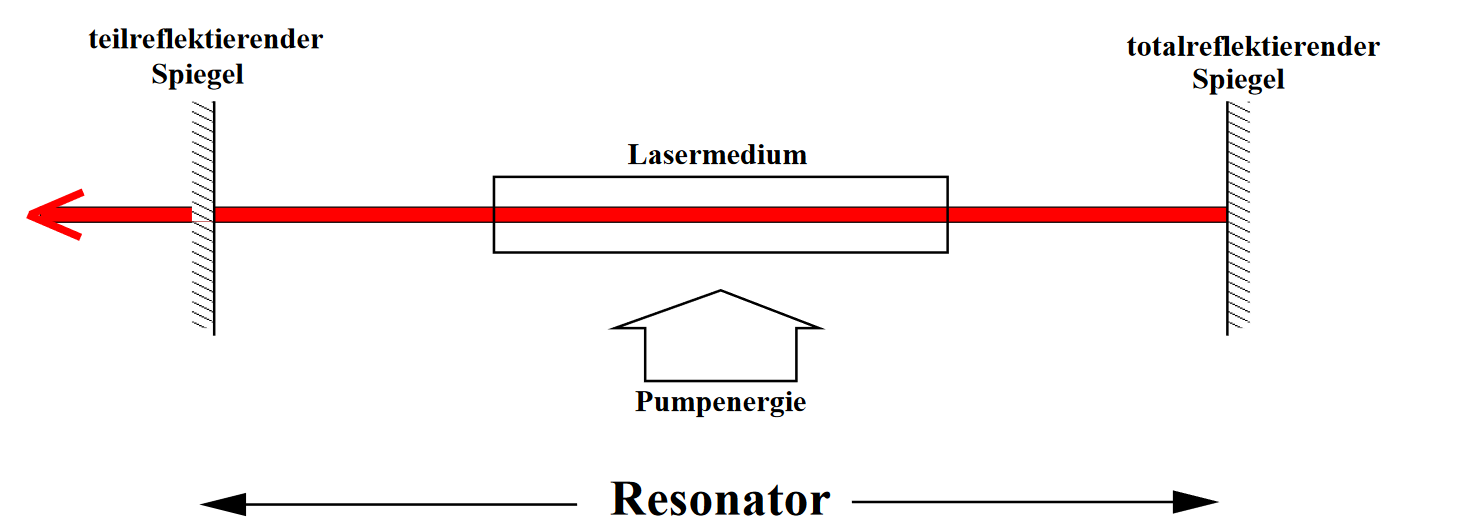
\includegraphics[width=\linewidth-100pt,height=\textheight-100pt,keepaspectratio]{content/Images/schema.png}
	\caption{Prinzipielle Funktionsweise eines Lasers \cite{V61}.}
	\label{fig:Aufbau}
\end{figure}
Ein Laser besteht im wesentlichen aus einem Resonator und einem Lasermedium und einer zugehörigen Pumpquelle. Das Lasermedium dient dabei zur Verstärkung des Lichtes und der Resonator sorgt für einen effektiv längeren Weg des Lichtes durch das Medium und die Pumpquelle versorgt das Lasermedium mit der für die Verstärkung notwendige Energie. 

\subsection{Der Resonator}
Der Resonator wird durch zwei gegenüber stehende Spiegel realisiert. Mindestens einer der Spiegel lässt etwas Licht durch und sorgt somit dafür, das das Licht den Laser verlassen kann. Bei den Spiegeln kann es sich jeweils um einen planparallelen Spiegel oder einem sphärischen Spiegel handeln. Sind beide sphärisch wird der Resonator als sphärischer Resonator bezeichnet und wenn beide planparallel sind als planparalleler Resonator. Damit der Resonator optisch stabil ist müssen die Verluste geringer sein als die Verstärkung durch das Lasermedium. Dies kann eintreten, wenn die Bedingung
\begin{equation}
	0 \leq \frac{r_1 -L}{r_1} \cdot \frac{r_2 -L}{r_2} \leq 1
\end{equation}
erfüllt ist. Hierbei sind $r_1$ und $r_2$ die Krümmungsradien der Spiegel und $L$ die Resonatorlänge, also der Abstand zwischen den Spiegeln. Damit sich die Stahlen optimal konstrucktiv überlagern muss weiterhin die im Resonator zurückgelegte Strecke ein vielfaches von der halben Wellenlänge des Lichtes sein. Diese Bedingung wird auch Resonanzbedingung genannt. Ist diese erfüllt bildet sich eine stehende Welle aus und das Licht wird maximal verstärkt. 

\subsection{Das Lasermedium}
\begin{figure}
	\centering
	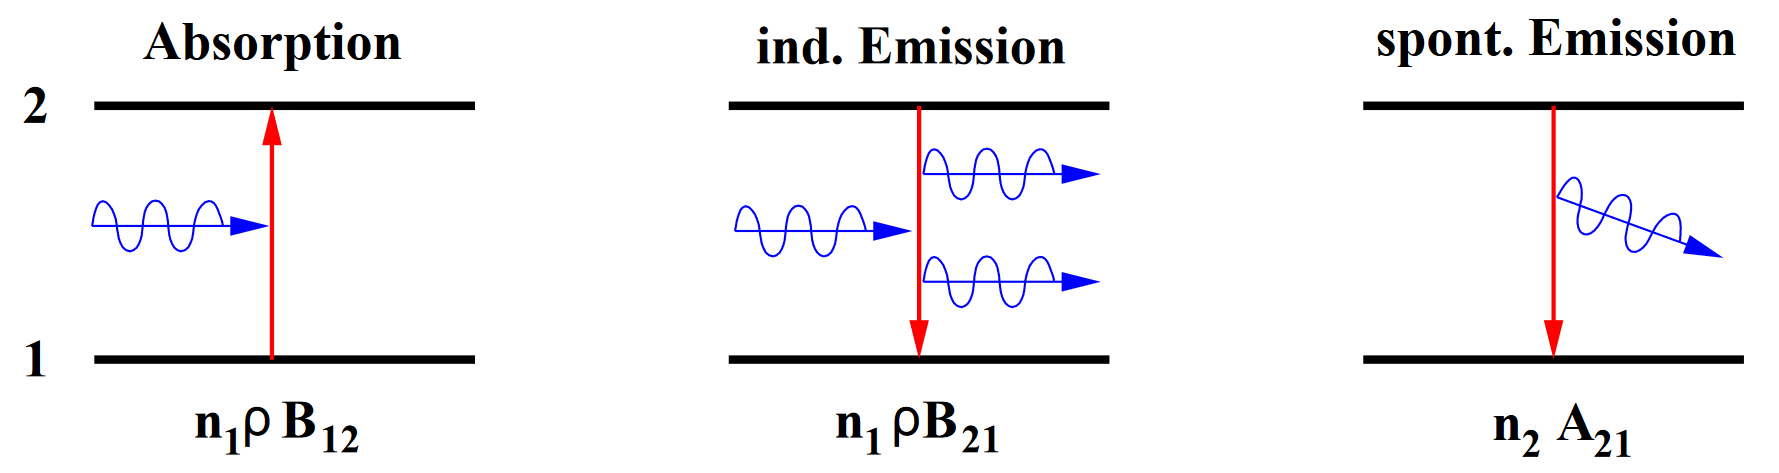
\includegraphics[width=\linewidth-100pt,height=\textheight-100pt,keepaspectratio]{content/Images/emission.png}
	\caption{Schemata für die Absorption und Emission bei einem 2-Niveau System \cite{V61}.}
	\label{fig:Aufbau}
\end{figure}
Das Lasermedium hat im einfachsten Fall einen angeregten Zustand und einen Grundzustand. Ein Photon hat nun drei Möglichkeiten diese Zustande zu beeinflussen. Einmal indem ein Photon mit entsprechender Energie absobiert wird und damit für einen Übergang auf das höhere Niveau sorgt (Absorbtion). Eine andere Möglichkeit besteht darin, dass das höhere Niveau spontan in das niedrigere Niveau übergeht und dabei ein Photon entsprechender Energie freigibt (spontane Emission). Jedoch ist es auch möglich, dass ein Photon mit der Energie des Energiedifferenz der Niveaus den Übergang vom höheren Niveau in das niedrigere Niveau stimuliert (indirekte Emission). 
Das besondere bei der indirekten Emission ist, dass das stimulierte Photon die selbe Ausbreitungsrichtung, Phase und Energie wie das stimulierende Photon besitzt. Dies ist der grundlegende Effekt der für einen Laser genutzt wird. In einem realen Lasermedium handelt es sich bei den verschiedenen Niveaus um die Besetzungsniveaus der Elektronenschalen der Atome. Damit es zu einer Verstärkung des Lichtes kommen kann muss mehr indirekt als emitiert werden als absorbiert wird. Da beide Prozesse gleich Wahrscheinlich sind kann dies durch eine höhere Besetzung des angeregten Zustandes als des Grundzustandes erreicht werden. Jedoch ist dies im thermischen Gleichgewicht nicht der Fall. Um dies dennoch zu erreichen muss durch Pumpen eine Besetzungsinversion geschaffen werden.

\subsection{Die Pumpquelle}
Das Pumpen kann auf verschieden Arten realisiert werden. 


\subsection{TEM-Moden}
Die Resonanzbedingung wird von mehreren Frequenzen erfüllt, sodass mehrere verschiedene Moden möglich sind. Die Moden werden bei einer zylindrischen Symmetrie werden mit $\text{TEM}_{plq}$-Mode ($text{TEM}=\text{transverse electromagnetic}$) bezeichnet. Die Ordnung der Mode wird in radialer Richtung mit $p$, in Winkelrichtung mit $l$ und entlang der Symmetrieachse (in $z$-Richtung) mit $q$ bezeichnet. Für die Intensität der Moden gilt
\begin{equation}
	I_{plq} = I_0 \cos^2 (l \varphi) \rho^2 \left[L_{p}^q\left(\frac{(2 \rho)^2}{1+Z^2} \right)\right] ^2 \exp\left(-\rho \right),
\end{equation}
wobei $L_{p}^q$ ein Laguerre-Polynom, $\rho=2 r^2 / w^2$, $w=w_0 \sqrt{1+\left(\frac{z \lambda}{\pi w_0^2}\right)^2}$ und $w_0$ der minimale Strahlradius ist.

Falls die Symmetrie durch z.B. Brewsterfenster gebrochen wird werden die Moden mit  $\text{TEM}_{mnq}$-Mode bezeichnet. Die Ordnung der Moden in $x$- und $y$-Richtung werden mit $m$ und $n$ bezeichnet. Für die Intensität der Moden gilt nun
\begin{equation}
I_{plq} = I_0 \left(\frac{w_0}{w}\right)^2 \left[H_m\left(\frac{\sqrt{2} x}{w}\right) \exp\left(\frac{-x^2}{w^2}\right) \right]^2 \left[H_n\left(\frac{\sqrt{2} y}{w}\right) \exp\left(\frac{-y^2}{w^2}\right) \right]^2,
\end{equation}
wobei $H_m$ ein Hermitesches Polynom ist.




\subsection{HeNe-Laser}

